\chapter{Oscillation Analysis}
\label{chap:OscillationAnalysis}

\section{Likelihood Calculation}
\label{sec:OscillationAnalysis_LLHCalc}

This analysis performs a joint oscillation parameter fit of the ND280,  and the SK atmospheric samples.

Once the Monte Carlo predictions of each beam and atmospheric sample has been built, following from \autoref{chap:SelsAndSysts}, a likelihood needs to be constructed. This is done by comparing the Monte Carlo prediction to ``data''. The data can consist of either an Asmiov Monte Carlo prediction, which is typically used for sensitivity studies, or real data. The Monte Carlo prediction is calculated at a particular point, \quickmath{\vec{\theta}}, in the model parameter space, \quickmath{N_{i}^{MC} = N_{i}^{MC}(\vec{\theta})}. Both the data and Monte Carlo spectra are binned, where the \quickmath{i^{th}} bin content is represented by \quickmath{N_{i}^{D}} and \quickmath{N_{i}^{MC}}, respectively. The bin contents for the beam near detector, beam far detector and atmospheric samples are denoted with \quickmath{ND}, \quickmath{FD} and \quickmath{Atm}, respectively. The binning index, \quickmath{i}, runs over all the bins within the sample and all samples with that set. Taking the beam far detector samples as example, it would run over all the reconstructed neutrino energy bins in all samples (FHC\quickmath{1\text{R}\mu}, RHC\quickmath{1\text{R}\mu}, etc.). The likelihood calculation between data and Monte Carlo for a particular bin follows a Poisson distribution, where the data is treated as a fluctuation of the simulation. 

Following the T2K analysis presented in \cite{Dunne2020-uf}, the likelihood contribution from the near detector also includes a Monte Carlo statistical uncertainty term, derived from the Barlow and Beeston statistical treatment \cite{Barlow1993-cc, Conway2011-go}. In addition to treating the data as a fluctuation of the Monte Carlo prediction, it includes a contribution from the likelihood that the generated simulation is a statistical fluctuation of the actual true simulation assuming infinite statistics. The technical implementation of this additional likelihood term is documented in \cite{t2k_tn_395}. The term is defined as,

\begin{equation}
  \frac{(\beta_{i}-1)^{2}}{2\sigma^{2}_{\beta_{i}}},
\end{equation}

where \quickmath{\beta_{i}} represents a scaling parameter for each bin \quickmath{i}, which is a value based on the amount of Monte Carlo statistics in a bin \cite{t2k_tn_395}. \quickmath{\sigma_{\beta_{i}} = \sqrt{\sum_{i} w_{i}^{2}}/N_{i}^{MC}}, and \quickmath{\sqrt{\sum_{i} w_{i}^{2}}} represents the sum of the square of the weights of the Monte Carlo events which fall into bin \quickmath{i}.

Additional contributions to the likelihood come from the variation of the systematic model parameters. For those parameters with well-motivated uncertainty estimates, a covariance matrix, \quickmath{V} describes the prior knowledge of each parameter as well as any correlations between the parameters. Due to the technical implementation, a single covariance matrix describes each ``block'' of model parameters, e.g. beam flux systematics. For simplicity, the covariance matrix associated with the \quickmath{k^{th}} block is denoted \quickmath{V^{k}}. This substitution results in \quickmath{\vec{\theta} = \sum_{k}^{N_{b}} \vec{\theta}^{k}} and \quickmath{V = \sum_{k}^{N_{b}} V^{k}}, for \quickmath{N_{b}} number of blocks describing: oscillation parameters, beam flux, atmospheric flux, neutrino interaction, near detector, beam far detector and atmospheric far detector systematics detailed in \autoref{sec:SelsAndSysts_Systs}. The number of parameters in the \quickmath{k^{th}} block is defined as \quickmath{n(k)}.

The final likelihood term is defined as,

\begin{align}
\label{eqn:Likelihood:Likelihood}
&-\ln(\mathcal{L}) = \\ 
& \sum_{i}^{\mathsf{ND bins}} N_{i}^{\mathrm{ND},MC}(\vec{\theta}) - N_{i}^{\mathrm{ND},D} + N_{i}^{\mathrm{ND},D}  \times \ln \left[ N_{i}^{\mathrm{ND},D}/N_{i}^{\mathrm{ND},MC}(\vec{\theta}) \right] + \frac{(\beta_{i}-1)^{2}}{2\sigma^{2}_{\beta_{i}}} \nonumber \\
& +  \sum_{i}^{\mathsf{FD bins}} N_{i}^{\mathrm{FD},MC}(\vec{\theta}) - N_{i}^{\mathrm{FD},D} + N_{i}^{\mathrm{FD},D}  \times \ln \left[ N_{i}^{\mathrm{FD},D}/N_{i}^{\mathrm{FD},MC}(\vec{\theta}) \right] \nonumber \\ 
& +  \sum_{i}^{\mathsf{Atm bins}} N_{i}^{\mathrm{Atm},MC}( \vec{\theta}) - N_{i}^{\mathrm{Atm},D} + N_{i}^{\mathrm{Atm},D} \times  \ln \left[ N_{i}^{\mathrm{Atm},D}/N_{i}^{\mathrm{Atm},MC}(\vec{\theta}) \right] \nonumber \\ 
& + \frac{1}{2} \sum_{k}^{N_{b}} \sum_{i}^{n(k)} \sum_{j}^{n(k)} (\vec{\theta}^{k})_{i} (V^{k})^{-1}_{ij} (\vec{\theta}^{k})_{j}. \nonumber
\end{align}

This is the value determined at each step of the MCMC to build the posterior distribution, as discussed in \autoref{chap:MarkovChainMonteCarlo}.

\iffalse
\subsection{Cross-Fitter Validation}
\label{sec:OscillationAnalysis_CrossFitter}

Alongside the analysis presented within this analysis, an alternative fitter \texttt{P-Theta}, has also been developing the analysis. For the purposes of this analysis, the main benefit of the alternative fitter is to validate the response to each parameter. 
\fi

\subsection{Likelihood Scans}
\label{sec:OscillationAnalysis_LLHScans}

Using the defintion of the likelihood presented in \autoref{sec:OscillationAnalysis_LLHCalc}, the response of each sample to a variation particular parameter can be studied. \autoref{fig:OscillationAnalysis_LLHScanOscPars} presents the variation of all the samples (beam and atmospheric) at SK. Each plot represents a ``scan'', where a particular parameter is scanned in some range. The ``data'' being used within the definition of the likelihood equation is built using the Asimov A oscillation parameter values defined in \autoref{tab:Theory_ParameterSets} alongside the pre-fit dial values as discussed in \autoref{sec:SelsAndSysts_Systs_Interaction}. Due to the correlations between oscillation parameters, the value of \quickmath{\chi^{2} \sim 1} does not equate to the typical \quickmath{1\sigma} sensitivity. However, it does give an indication of which samples response the strongest to a variation in the oscillation parameters. The point at which the likelihood tends to zero illustrates the value of the parameter used to build the Asimov data prediction. The likelihood scans only include the sample response and ignore the penalty contribution term from the variation of the parameter.

\begin{figure}[h]
  \begin{subfigure}[t]{0.5\textwidth}
    \includegraphics[width=\textwidth, trim={0mm 0mm 0mm 0mm}, clip,page=4]{Figures/OA/LLHScans_Osc.pdf}
    \subcaption{\quickmath{\sin^{2}(\theta_{23})}}
  \end{subfigure}%
  \begin{subfigure}[t]{0.5\textwidth}
    \includegraphics[width=\textwidth, trim={0mm 0mm 0mm 0mm}, clip,page=7]{Figures/OA/LLHScans_Osc.pdf}
    \subcaption{\quickmath{\Delta m^{2}_{23}}}
  \end{subfigure}
  \begin{subfigure}[t]{0.5\textwidth}
    \includegraphics[width=\textwidth, trim={0mm 0mm 0mm 0mm}, clip,page=8]{Figures/OA/LLHScans_Osc.pdf}
    \subcaption{\quickmath{\delta_{CP}}}
  \end{subfigure}%
  \begin{subfigure}[t]{0.5\textwidth}
    \includegraphics[width=\textwidth, trim={0mm 0mm 0mm 0mm}, clip,page=5]{Figures/OA/LLHScans_Osc.pdf}
    \subcaption{\quickmath{\sin^{2}(\theta_{13})}}
  \end{subfigure}
  \begin{subfigure}[t]{0.5\textwidth}
    \includegraphics[width=\textwidth, trim={0mm 0mm 0mm 0mm}, clip,page=3]{Figures/OA/LLHScans_Osc.pdf}
  \end{subfigure}
  \caption{The response of the likelihood, as defined in \autoref{sec:OscillationAnalysis_LLHCalc}, illustrating the response of the samples to the oscillation parameters. \delmsqsol and \sinsqsol are negated because these samples have no sensitivity to those parameters. The Asimov data set is built using the pre-fit dial values assuming Asimov A oscillation parameters defined in \autoref{tab:Theory_ParameterSets}. \finish{Need finer binning on delmsq23}}
  \label{fig:OscillationAnalysis_LLHScanOscPars}
\end{figure}

The response to \delmsqatm is much larger in beam samples, specfically \quickmath{\mu}-like samples, compared to atmospheric samples. This is in agreement with what we observe in the comparison of the data fit contours presented in \autoref{fig:NeutrinoOscillationPhysics_AtmosphericParamContour}. However, we know that the determination of the mass hierarchy is signficantly enhanced when using the atmospheric samples due to them transitioning through the Earth's core. A similar story is seen in the response to \sinsqatm. However, the disparity is much smaller. Summing the atmospheric sample likelihood contributions, the responce becomes close to that of the beam samples. The only samples which respond to the \sinsqreac parameter are the electron-like beam samples. Consequently, no increase in sensitivity beyond that of the T2K-only analysis is expected. The \delmsqsol and \sinsqsol are not considered as there is simply no sensitivity in any sample considered within this analysis.

In addition to the oscillation parameters, the response to the systematic model parameters can also be considered. Due to the correlated cross section model, the most informative 
